\chapter{Cognitive Communication}
\label{chap:wav}

We are currently in the phase of conceptualizing the requirements of the fifth generation (5G) of mobile wireless systems. One of the major goals is to improve the areal capacity ($\SI{}{bits/s/m^2}$) by a factor of 1000 \cite{Andrews14}. \tc{To this end, an extension to the already allocated spectrum is of paramount importance.} 
Recently, the spectrum beyond \SI{6}{GHz}, which largely entails the millimeter wave is envisaged as a powerful source of spectrum for 5G wireless systems. However, the millimeter wave technology is still in its initial stage and along with complex regulatory requirements in this regime, it has to address several challenges like propagation loss, low efficiency of radio frequency components such as power amplifiers, small size of the antenna and link acquisition \cite{Rapp13}. Therefore, in order to capture a deeper insight of its feasibility in 5G, it is essential to overcome the aforementioned challenges in the near future.

\tc{Besides the spectrum beyond \SI{6}{GHz}, an efficient utilization of the spectrum below \SI{6}{GHz} presents an alternative solution. The use of the spectrum in this regime (below \SI{6}{GHz}) is fragmented and statically allocated, leading to inefficiencies and the shortage in the availability of spectrum for new services.} However, it is possible to overcome this scarcity if we manage to utilize this radio spectrum efficiently. In this perspective, \tc{cognitive radio (CR) is foreseen as one of the potential contenders that addresses the spectrum scarcity problem. Since its origin by Mitola \textit{et al.} in 1999, this notion has evolved at a significant pace, and consequently has acquired certain maturity.} However, from a deployment perspective, this technology is still in its preliminary phase. In this view, it is necessary to make substantial efforts that enable the placement of this concept over a hardware platform.

An access to the licensed spectrum is an outcome to the paradigm employed by the \tc{secondary user (SU)}. Based on the paradigms described in the literature, all CR systems that provide dynamic access to the spectrum mainly fall under three categories, namely, interweave, underlay and overlay systems \cite{Goldsmith09}. In \tc{interweave systems (ISs)}, the SUs render an interference-free access to the licensed spectrum by exploiting spectral holes in different domains such as time, frequency, space and polarization, whereas underlay systems enable an interference-tolerant access under which the SUs are allowed to use the licensed spectrum (e.g. Ultra Wide Band) as long as they respect the interference constraints of the primary receivers (PRs). Besides that, overlay systems consider the participation of higher layers for enabling the spectral coexistence between two or more wireless networks. Due to its ease of deployment, the IS is mostly preferred not only for performing theoretical analysis but also for practical implementation as well. Motivated by these facts, this paper focuses on the performance analysis of the ISs from a deployment perspective. 

\section{Cognitive radio}
\begin{itemize}
\item Mitola's concept
\item Dynamic spectrum access: A cognitive radio application for resolving spectrum scarcity
\item Cognitive radio in relation to software defined radio
\end{itemize}

\section{Paradigms for cognitive radio}
\subsection{Interweave systems}
\subsection{Underlay systems}
\subsection{Overlay systems}



%\section{Introduction}

%The hardware for radio devices changed dramatically in the last decades and so did the development of waveforms. In former times, waveform development consisted mainly of designing electronic circuits for specific waveforms. Nowadays, waveform development means programming on different processing units like \acp{GPP}, \acp{DSP} or \acp{FPGA}. In addition the way of programming changed from a platform specific to a platform independent development. These approaches deal with a trade-off between efficient platform specific code on the one hand and a portable platform independent code on the other. This chapter gives an overview of the existing and common ways for waveform development and describes in more detail a new approach of the model-based waveform development under the aspect of portability. It furthermore gives a closer look into the performance overhead of generated code by measuring the processing time as well as the logic resources and compares it with hand-written code.

%\section{Use Case}

%\subsection{Platform Specific Development}

%Implementing applications for a specific SDR platform is the traditional way of waveform development. The code is optimized for the underlying processing element and the platform specific tools are used to maximize performance in sense of speed, size and power. Although this is a high-performance approach, existing optimized codes can hardly be ported to other processing elements. If you additionally think of porting the code from \ac{GPP} to \ac{FPGA} this means a complete rewriting of the algorithms.

%\subsubsection{Code Development on Processors}
%For processors, a lot of programming languages exist, but only a few are used for digital signal processing  and embedded systems. This is due to the performance constraints in power, speed and code size. Benchmarks show that C and C++ belong to the most powerful languages in that field \cite{prechelt_comparison}, \cite{language_bench}. However, it has to be mentioned that benchmarks for dedicated programming languages have only limited significance. This is due to the fact that benchmarks for processing times or cycles measure not the language itself but the application behind. Nevertheless, C and C++ are, according to the results from \cite{prechelt_comparison} and \cite{language_bench}, the choices of the \ac{DSP} industry. Figure \ref{fig:dsp_market_share} shows the DSP vendor market shares in 2006. It is remarkable that development environments from these vendors only support C based and assembly languages. According to this result, this work focuses only on C, C++ and optimized libraries written in Assembler.

\begin{figure}[htb]
	\centering
		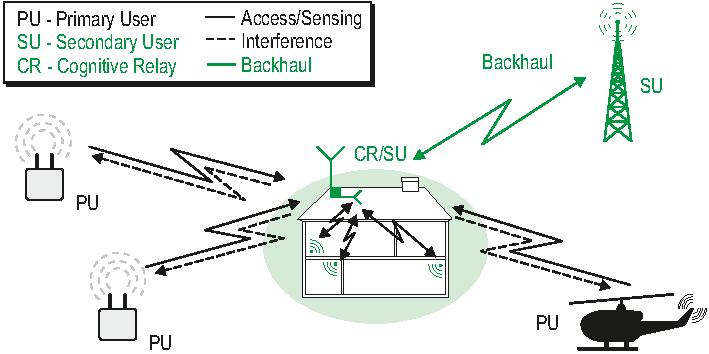
\includegraphics[width = \columnwidth]{../kapitel02/figures/wo_channels_CR_Scenario_farbig_general}
	\caption{A scenario demonstrating the interaction between the PU and the CR.}
	\label{fig:dsp_market_share}
\end{figure}

%Furthermore, a still recent topic is the choice between the languages C, C++ and assembly. The big advantage and the main reason why assembly languages are still used is the direct mapping from language to processor instruction. This mapping gives the programmer any control to optimize the code in the sense of speed and size. Even if the performance constraints are relaxed, small execution times lead to a decrease of the clock frequency and to a lower power consumption. Nevertheless, high-level languages\index{High-Level Language} like C became more and more popular in embedded systems due to three main reasons \cite{dsp_high_level}:
%
%\begin{itemize}
%	\item better portability between hardware platforms
%	\item protection of the investment in program code
%	\item reduced development time
%\end{itemize}
%
%In modern systems, there has to be a trade-off between high-level and low-level programming languages. On the one hand the application should be executed as fast as possible while on the other hand the shrinking time to market calls for portable code. Therefore, almost any vendor for integrated development environments provides user guides and tutorials for C optimizations ( \cite{anderson_optimizing_C}, \cite{ti_opt_C} or \cite{amd_opt_C}). They also claim that well written, efficient and platform independent C code is appropriate for most applications due to platform optimized compilers. The code section represented in listing \ref{source_01} calculates the dot product for two variables in simple C. Listing \ref{unopt_ass_01} shows the assembly code that is produced by the compiler without \index{Optimization}optimizations. By enabling the compiler optimizations, the code is reduced to only a few lines, shown in listing \ref{opt_ass_01}. Due to the fact that the code is written clearly, the compiler is able to optimize it and to use the platform specific architecture. It can calculate two \ac{MAc} operations and simultaneously load two data elements in one single cycle. This example was written for Analog Devices Blackfin DSP and compiled with VisualDSP++.
%
%
%\begin{lstlisting}[columns=flexible,caption=Example code in C,label=source_01]
%for (i=0; i< 150; i++){
%  dotp += b[i] * a[i];
%  sqr  += b[i] * b[i];
%  }
%\end{lstlisting}
%
%\pagebreak
%
%\begin{lstlisting}[caption = Unoptimized assembler code,abovecaptionskip = 0mm,belowcaptionskip = -5mm, label=unopt_ass_01]
%\end{lstlisting}
%\begin{multicols}{2}
%\begin{lstlisting}[columns=flexible]
%[FP+ -8] = R7;
%._ P1L1:
%  R3 = [FP+ -8];
%  R2 = 150 (X);
%  CC = R3 < R2;
%  IF !CC JUMP ._P1L3;
%  R3 <<= 1;
%  P2 = R3;
%  P0 = [FP+ 8];
%  P0 = P0 + P2;
%  R1 = W[P0+ 0] (X);
%  R0 = [FP+ -8];
%  R0 <<= 1;
%  P1 = R0;
%  P2 = [FP+ 12];
%  P2 = P2 + P1;
%  R7 = W[P2+ 0] (X);
%  R7 *= R1;
%  R1 = [FP+ -4];
%  R0 = R1 + R7;
%  [FP+ -4] = R0;
%  R3 = [FP+ -8];
%  R3 <<= 1;
%  P0 = R3;
%  P1 = [FP+ 12];
%  P1 = P1 + P0;
%  R1 = W[P1+ 0] (X);
%  R7 = [FP+ -8];
%  R7 <<= 1;
%  P2 = R7;
%  P1 = [FP+ 12];
%  P1 = P1 + P2;
%  R3 = W[P1+ 0] (X);
%  R3 *= R1;
%  R1 = [FP+ 16];
%  R7 = R1 + R3;
%  [FP+ 16] = R7;
%  R3 = [FP+ -8];
%  R3 += 1;
%  [FP+ -8] = R3;
%  JUMP ._P1L1;
%\end{lstlisting}
%\end{multicols}
%
%\begin{lstlisting}[caption=Optimized assembler code,label=opt_ass_01]
%LSETUP (._P1L2 , ._P1L3-8) LC0=P1;
%._P1L2:
%  A1+= R0.H*R0.H, A0+= R0.L*R0.H (IS)
%      || R0.L = W[I1++]
%      || R0.H = W[I0++];
%			
%._P1L3:
%\end{lstlisting}
%
%There are several other ways of optimizing C code beside the optimizing abilities of the compiler. However, \cite{lee_opt_C} claims that even an optimum assembler code is merely \SI{10}{\%} faster than a well written C code. In addition the rising speed of processors made it possible to pass by the assembly language in most cases. If the code is still too slow, despite of being well written, the positive impact of the Pareto Principle\index{Pareto Principle} can be applied. It says that small code portions (\SI{10}{\%} - \SI{20}{\%}) are consuming most (\SI{80}{\%} - \SI{90}{\%}) of the system resources \cite{pareto}. The performance critical code segments can be identified easily and tuned with optimized assembler code. This can be done for example by applying vectorization or parallelization of the underlying processor. However, these code segments can hardly be ported to other platforms.
%
%A similar discussion about the choice between C and assembly language can be observed in the choice between C and C++. C++ is often seen as slow, inefficient and too large for embedded systems. However, these are assumptions that must not be true, due to the fact that obviously C++ is just a superset of the C language. This means that implementing in C and compiling with a C++ compiler should not produce any overhead. Unfortunately that is not really true. In \cite{dsp_high_level} this overhead was investigated by compiling C benchmark programs with the TASKING DSP563xx C and C++ compilers and comparing the speed and size. The result was that the execution speed decreased by no more than \SI{1.6}{\%} while the code size growed by no more than \SI{6.8}{\%}. C++ features are not consuming much more space than elements in C do if they are well designed. The key issue for writing efficient high-level code (independent of C or C++) is that the developer is aware of the functionality at machine code level and the work of the compiler.
%
%\subsubsection{Code Development on \acp{FPGA}}
%An \ac{FPGA}\index{FPGA} has to be programmed different from a microprocessor or \ac{DSP}, due to its underlying hardware structure (see section \ref{sec:dsp_sdr}). While processors are implemented in assembly language, which can be mapped to the binary machine code instructions, the \ac{FPGA} and its underlying logic is represented by an \ac{HDL}. The \ac{HDL}\index{HDL} is a formal description of the digital logic with reference to the timing behavior. In the beginnings of \acp{HDL} only representations for either the logical behavior or the structure existed. This changed in the 1980s when two new languages appeared, representing the logical and structural behavior: Verilog and VHDL. These languages are still dominating the FPGA world, but their distribution is locally different. While Verilog\index{Verilog} is the most popular \ac{HDL} at the US west coast and Asia, VHDL\index{VHDL} is the preferred language in Europe and the US east coast \cite{baese}. There are various discussions about the advantages and disadvantages of these two \acp{HDL} and several papers compare them based on example applications \cite{verilog_vs_vhdl01}, \cite{verilog_vs_vhdl_02}. The choice between Verilog and VHDL depends lastly not on technical capabilities but on personal references, tool capability and existing code to reuse. 
%
%\subsubsection{Portability with platform specific development}
%Platform specific waveform development is, as indicated by the name, dependent on the underlying processing element. C and C++ code can be ported from one GPP to another without a major decrease in performance. But this is only true under the condition that the operating systems are not changing. The porting of DSP code depends on the underlying architecture. The port from a floating point processor to a fixed point processor forces the compiler to translate every floating point instruction into fixed point instructions with exception handling in case of overflows. Furthermore, a program with processor specific intrinsics can not be ported to a new platform. The sections of the code with the platform specific commands have to be rewritten. Although C and C++ are high level programming languages, there is no assurance that they can be ported without modifications or loss in performance. This is even more dramatic when porting \ac{HDL}. The choice of language is predetermined by the platform developer and provider of the board support kit. Therefore, a specific language has to be used and code can not be ported if it is available in the wrong language.
%
%\subsection{GNU Radio}
%\label{GNURadio}
%\index{GNU Radio}
%
%GNU Radio is an open source project for building waveforms for software defined radios \cite{gnu_radio_art}. The idea is the interpretation of a waveform as multiple components that are composed together. The components with an input and output port build the signal processing blocks, while blocks with only input or output ports can be named sinks or sources. Therefore, the GNU Radio library supports hundreds of components written in C++. The connection between blocks and the creation of waveforms is accomplished by building a flow graph in Python that holds the components as primitives. The code example \ref{gnuradio_01} works as an ``Hello World'' tutorial for GNU Radio. It generates two sine waves with a frequency of \SI{350}{Hz} and \SI{400}{Hz}, adds them and passes the output to the sound card. In lines 13 to 16 the components are defined and configured. The simplicity of GNU Radio can be seen on line 18 and 19. The components can be connected with the instruction \texttt{connect()}. The whole scheduling and necessary inter-process communication is done by GNU Radio itself. 
%
%\begin{lstlisting}[language=Python,columns=flexible,caption=Dial tone example in GNU Radio,label=gnuradio_01]
%#!/usr/bin/env python
% 
%from gnuradio import gr
%from gnuradio import audio
%
%class my_top_block(gr.top_block):
%  def __init__(self):
%    gr.top_block.__init__(self)
%
%    sample_rate = 32000
%    ampl = 0.1
%
%    src0 = gr.sig_source_f(sample_rate, gr.GR_SIN_WAVE, 350, ampl)
%    src1 = gr.sig_source_f(sample_rate, gr.GR_SIN_WAVE, 440, ampl)
%    add  = gr.add_ff()
%    dst  = audio.sink (sample_rate, "")
%        
%    self.connect (src0, (add,0))
%    self.connect (src1, (add,1))
%    self.connect (add, dst)
%
%if __name__ == '__main__':
%  try:
%    my_top_block().run()
%  except KeyboardInterrupt:
%    pass        
%\end{lstlisting}
%
%Despite the comprehensive signal processing library, GNU Radio was only used by few developers through the beginning years. In 2004 Ettus Research LLC released the first version of the USRP as an RF front end that can be connected directly with GNU Radio. Therefore, the community of developers for GNU Radio increased. The next step in the evolution of GNU Radio was the development of a tool, named as \ac{GRC}\index{GRC}, which graphically connects and configures components to a flow graph. The equivalent example from listing \ref{gnuradio_01} is shown in the \ac{GRC} environment in figure \ref{fig:gnuradio_grc}. The graphical flow graph can automatically generate the Python code where lower programming experience for SDR developers is demanded. 
%
%\begin{figure}[htbp]
%	\centering
%		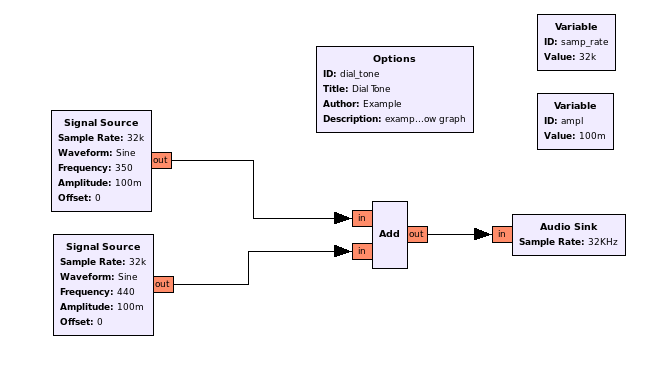
\includegraphics[width=1.00\textwidth]{../kapitel02/figures/gnuradio_grc.png}
%	\caption{Dial tone example in the GNU Radio Companion}
%	\label{fig:gnuradio_grc}
%\end{figure}
%
%GNU Radio composes the waveform with a flow graph and allows the developer to build waveforms that are independent of the underlying hardware. Nevertheless they are not independent of the underlying operating system. In simple terms GNU Radio waveforms are portable between processors that run Linux operating systems. It has to be mentioned that ports of GNU Radio were only successful from a GPP to another GPP. Even if there have been ports to various hardware platforms like Sony's Playstation 3 \cite{gnu_radio_web} and the BeagleBoard \cite{open_sdr}, it has to be mentioned that GNU Radio only ran on the GPP part of these multi core platforms, neither on DSPs nor on FPGAs.
%
%
%\subsection{Software Communication Architecture}
%\label{sec:SCA}
%
%\subsubsection{History of the Software Communication Architecture}
%Waveform development and portability aspects are also enforced by U.S. military. It maintains hundreds of different legacy radios, which are neither upgradeable nor compatible to each other. In parallel the processor capabilities increased in the last two decades according to Moore's Law \cite{moores_law}, \cite{moores_law_2}. This claims that the number of transistors that can be placed on the same area is doubled every other year. The development in chip technology and in the DSP capability resulted in a shift of the borders between analog and digital domain of a radio towards the antenna as mentioned in section \ref{sec:mot}. Therefore, the \ac{JTRS} \ac{JPO} was founded in 1997 to develop a family of the next generation of reconfigurable software-based tactical radios. This system should increase the flexibility and interoperability among the legacy radio systems to reduce the costs for maintenance and to supply and provide the ability to upgrade not only hardware parts but also the software of the radio. The first milestone in this effort was the definition of a common software architecture for these radios: The \ac{SCA}\index{SCA}. To accomplish the \ac{JTRS} project goals, the SCA was intended to support portability between SCA compliant implementations, and to use already established frameworks and architectures from the industry. This should result in minimizing the development time due to reuse of waveform components.
%
%\subsubsection{Operating Environment}
%\index{Operating Environment}
%The \ac{OE} builds the interface between a waveform component and the radio \cite{SCA_Tutorial_VT}. One part of it is the operating system of the radio. To be independent of the underlying hardware and the operating system, the \ac{OE} provides several interfaces for the waveform components to communicate with its environment: These are the interfaces provided by the \acl{CF} and CORBA\index{CORBA} and additionally the \ac{AEP}\index{AEP}. The access points for the application to the operating system are shown in figure \ref{fig:OE}.
%
%\begin{figure}
%	\centering
%		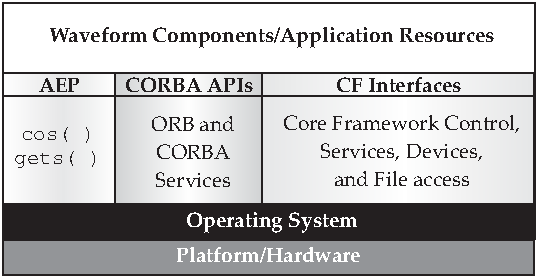
\includegraphics[]{../kapitel02/figures/operating_environment.pdf}
%	\caption{Operating Environment with the connections to the platform and the waveform}
%	\label{fig:OE}
%\end{figure}
%
%\subsubsection{Core Framework}
%\index{Core Framework}
%
%The \ac{CF} provides interfaces to the operating system, which can be used by the waveform or other applications running on the \ac{OE}. The interfaces give access to various services like the installation, management or configuration of a waveform. Another purpose of the interfaces is to abstract the underlying hardware. Therefore, four classes of \ac{CF} interfaces are specified:
%
%\begin{itemize}
%	\item Base Application Interfaces
%	\item Base Device Interfaces
%	\item Framework Control Interfaces
%	\item Framework Service Interfaces
%\end{itemize}
%
%The base application interfaces provide access to waveform components like initializing or releasing, configuring or querying the properties of the different components for testing purposes. The software components for access to the hardware resources are called devices, where the basic device interfaces allow interaction with the physical hardware devices on the radio. The framework control interfaces provide a radio wide control of services like installation, deployment or management while the framework service interfaces supply additional services like management of file systems.
%
%\subsubsection{CORBA}
%\index{CORBA}
%
%The \ac{CORBA} is an open specification for mechanisms calling objects from other processes per remote. The specific characteristic of \ac{CORBA} is, that these objects can run under different operating systems or on different processor architectures and that they can even be implemented with a different programming language. The remote calls can not be distinguished in the implementation from local calls. This is the main reason of the inclusion of \ac{CORBA} in the \ac{SCA} due to the fact that waveform components should exchange information without knowledge of the underlying operating systems and transport mechanisms. Nevertheless, \ac{CORBA} has also some technical restrictions. The most important is the complexity and the size of its \acp{API}, which are quite larger than necessary \cite{rise_fall_corba} and therefore not well suited to an embedded system. To circumvent this, the \ac{SCA} dictates the use of minimumCORBA, standardized by the \acl{OMG}. MinimumCORBA is a subset of \ac{CORBA} designed for systems with limited resources.
%
%\subsubsection{Application Environment Profile}
%\index{AEP}
%
%The \ac{IEEE} and The Open Group specified \acp{API} between application and operating system under the name \ac{POSIX}. The \ac{SCA} \cite{SCA222} dictates with the \ac{AEP} a subset of \ac{POSIX} with 256 \acp{API}. This includes for example mathematical operations like \lstinline[language=C]!cos()!, \lstinline[language=C]!sin()!, \lstinline[language=C]!tan()! or string operations like \lstinline[language=C]!gets()!, \lstinline[language=C]!getchar()!. Due to the fact that these interfaces are standardized, the access from the waveform component to the underlying operating system, is portable without the use of the \ac{CF} or \ac{CORBA}.
%
%
%\subsubsection{Domain Profile}
%\index{Domain Profile}
%
%Beside the aspect of portability, an additional requirement of SCA compliant radios is the reconfigurability. Therefore, the Domain Profile provides an essential description of the platform and the waveform application. The Domain Profile consists of several description files written in \ac{XML}. These files describe:
%\begin{itemize}
%	\item the various hardware devices
%	\item the waveform components
%	\item the deployment
%	\item the connections between components
%	\item the properties of components and devices 
%\end{itemize}
%
%With this information the SCA-compliant radio is able to deploy a waveform, independent of the underlying hardware.
%
%\subsubsection{SCA-compliant waveform development}
%The development of an SCA-compliant waveform requires a good understanding of the \ac{SCA} \ac{CF}. However, there are tools that make it easier for waveform developers. Beside professional tools like SCARI \cite{scari:website}, Spectra \cite{spectra:website} or Component Enabler \cite{ce:website}, the Open Source project Ossie \cite{ossie:website} builds a complete SCA framework with code generation. It already supports interfaces to the USRP and the USRP2 and was ported to environments including FPGAs \cite{ossie_fpga} and DSPs \cite{ossie_omap}. 
%
%\section{Model-Based Development}
%\label{sec:mbd}
%
%\subsection{OMG's Model Driven Architecture}
%\index{MDA}
%The \ac{OMG} is a non-profit international computer industry consortium for standardizing distributed object-oriented software systems as well as model-based developments. It created the development and the standardization of modeling architectures like the Unified Model Language (UML) as well as middleware solutions like \ac{CORBA}, which is described in section \ref{sec:SCA}. In 2001 \ac{OMG} adopted the \ac{MDA}, which can be seen as an approach for the usage of models in software development to provide portability, interoperability and reusability \cite{MDAGuide}. These goals can be achieved by the concept of separating the functionality of an application from the capabilities of the underlying platform. The fundamental idea is to initiate an iterative process in developing models of a specific system and to extend these models in a last step to an application running on a platform. Therefore, the MDA suggests to start the development with a \ac{CIM}\index{CIM} for the requirements of the system, but which is independent of the way how the system is built. The first step of an implementation is the \ac{PIM}\index{PIM}. This is a model that describes the system but does not show details of its use of any platform. The first implementation with platform details is realized in the \ac{PSM}\index{PSM}. As the name implies, this illustrates how the system uses the underlying platform to fulfill the functionality and the requirements specified in the \ac{CIM}. The step from one model to another is called transformation. The \ac{MDA} does not define a specific method for the transformation. However, it gives examples from all manual transformations up to fully automated transformations \cite{MDAGuide}.
%
%In contrast to the \ac{MDA}, the \ac{SCA} is also defining its waveforms in a platform independent manner but models the platform itself in a Platform Specific Model with the Domain Profile. The transformation for this \ac{PSM} to executable code running in real-time on the SDR platform should be done with the Core Framework and \ac{CORBA}. However, \ac{CORBA} comes with overhead in processing time and memory usage and is therefore not the best choice for the baseband processing. Due to this, the MDA should be reinterpreted to fit the needs of baseband processing on heterogeneous hardware architectures.
%
%\subsection{A new interpretation of the MDA} 
%The introduced models \ac{CIM}, \ac{PIM}, and \ac{PSM} build the basis of the \ac{MDA} and should should be maintained. However, the interpretation should be more application specific concerning the air interface. The \ac{CIM} that should describe the requirements independent of the implementation is actually the specification of the waveform. While most specifications for industry waveforms are open to public (e.g. specifications of \ac{IEEE} or \ac{ETSI}), this is not the case for military waveforms. These waveforms were built for legacy devices where the baseband data were processed with hardware. The specifications are not open and in some cases not even existent. This results in a lot of work for reengineering and creating the \ac{CIM} when the waveform should be supported by an SDR. The transformation to the \ac{PIM} can be accomplished by implementing the waveform without platform specific aspects. Therefore high-level languages can be used, which support good debug and simulation features. The \ac{PIM} is a model for the implementation of the waveform's functionality. This includes for example the realization of the synchronization schemes or the design of the digital filters. The step to the \ac{PSM} is done by extending the \ac{PIM} with platform specific aspects. These can be infrastructural platform aspects like the data buses on the system or the configuration of the RF front ends and \acp{ADC}. Further platform specific aspects are processor specific issues like the adaption of algorithms for fixed-point representations. The last transformation from the \ac{PSM} to an executable code is done automatically with code generation tools like \emph{Real Time Workshop} or \emph{HDL Coder} from the company The Mathworks and processor specific compilers like \emph{Visual C Compiler} from Microsoft, \emph{Code Composer Studio Compiler} from \ac{TI} or \emph{Intel Parallel Studio}. Another example for this use of the \ac{MDA} is described in \cite{schober_mda} and \cite{nagel_tetra}. Figure \ref{fig:mda_structure} summarizes the steps from CIM to Code.
%\begin{figure}
%	\centering
%		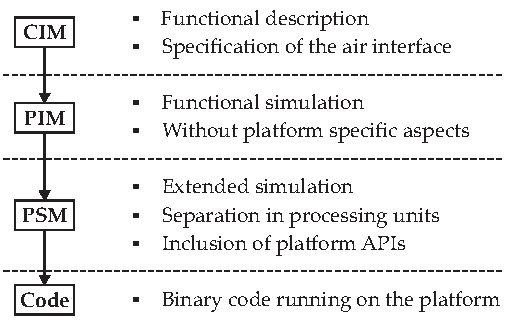
\includegraphics[]{../kapitel02/figures/mda_structure.pdf}
%	\caption{Overview of the models, which are defined by the MDA}
%	\label{fig:mda_structure}
%\end{figure}
%
%
%
%\subsection{Model-Based Design with Simulink}
%\index{Simulink}
%Simulink \cite{simu_ug} is a visual programming language, which allows engineers to model dynamic systems. It provides hundreds of blocks, which generate, process and consume data. Furthermore, Simulink supports extensions to generate code in the languages C, C++, Verilog and VHDL. It is therefore used in this work for waveform development. This section should give an overview of the principles of Simulink and its extensions to code generation.
%
%\subsubsection{Simulation}
%In introductions to programming languages the ``Hello World'' example is used very often. However, this does not make sense for a visual programming language that is used for digital signal processing. A better example is the ``dial tone'' example from section \ref{GNURadio}. The generation and processing of two sine waves gives an overview of the necessary parameters and configurations.
%
%
%\begin{figure}
%	\centering
%		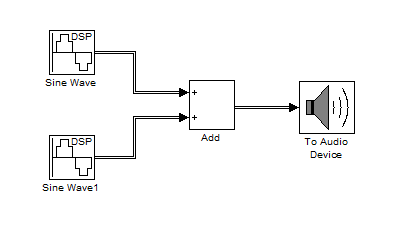
\includegraphics[width=0.75\textwidth]{../kapitel02/figures/dial_tone_simu.PNG}
%		\caption{Dial tone example in Simulink}
%	\label{fig:dial_tone_simu}
%\end{figure}
%
%Figure \ref{fig:dial_tone_simu} shows the dial tone example in a Simulink environment. The blocks require information about the sample time as well as frequency and magnitude of both sine waves. This does not differ from the \ac{GRC} model described in section \ref{GNURadio}. The difference is in the optional handling of the data. While GNU Radio considers the data flow as a stream without the knowledge of the actual processing, Simulink provides the opportunity to parameterize the size of vectors in the initialization phase. This results in new degrees of freedom. While the processing on single values (sample-based)\index{Sample-based processing} minimizes latency, the throughput is decreased due to the \ac{ISR} after each sample. Working on multiple values (frame-based)\index{Frame-based processing} increases the latency and the memory usage but optimizes the performance with respect to execution time. Figure \ref{fig:sample_frame} clarifies this relation.
%
%\begin{figure}
%	\centering
%		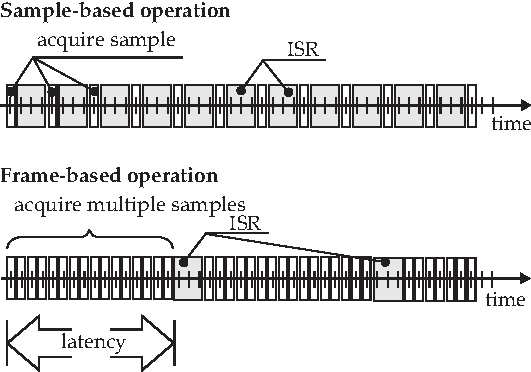
\includegraphics{../kapitel02/figures/sample_frame.pdf}
%	\caption{Comparison of latency and throughput for sample-based and frame-based processing}
%	\label{fig:sample_frame}
%\end{figure}
%
%
%\subsubsection{Code Generation from Simulink to C/C++}
%\label{sec:codegen}
%Real Time Workshop \cite{rtw_ug} and Real Time Workshop Embedded Coder \cite{rtwec_ug} extend Simulink's functionalities with the ability to generate C and C++ code for real-time systems. For building executable models, it is not only necessary to generate the code for the algorithmic function. This code must also support run time interfaces as well as scheduler and memory transfer. Therefore, the following steps are executed:
%
%\begin{itemize}
%	\item \textbf{\texttt{ModelInitialize}}: Initializes the code for the run-time interface and the model. This includes  allocation of memory and data that can be calculated prior to the execution of the algorithm.
%	\item \textbf{\texttt{ModelOutput}:} Calls all blocks in the model that have a sample hit at the current time and 
%	produce their output. The output follows a given simulation time step.
%	\item \textbf{\texttt{ModelUpdate}:} Calls all blocks in the model that have a sample hit at the current point in time and update their discrete states.
%	\item \textbf{\texttt{ModelTerminate}:} Terminates the program if it is designed to run for a finite time. It deallocates memory and can write data to a file.
%\end{itemize}
%
%The pseudo code in listing \ref{rtw_01} shows how these functions are integrated in the generated code. 
%
%\begin{lstlisting}[language=C,columns=flexible,caption= Structure of a generated model in pseudo code \cite{rtw_ug},label=rtw_01]
%rtOneStep()
%{
%  //Check for interrupt overflow
%  //Enable "rt_OneStep" interrupt
%  ModelOutputs();    // Major time step.
%  LogTXY();          // Log time, states and root outports.
%  ModelUpdate();     // Major time step. 
%}
%
%main()
%{
%  ModelInitialize();
%  //including installation of rtOneStep as an 
%  //interrupt service routine for a real-time clock
%  
%  while(time < final time){
%  	rt_OneStep();
%    //Background task
%    }
%  ModelTerminate();
%  //Mask interrupts (Disable rt_OneStep() from executing.)
%  //Complete any background tasks.
%  //Shutdown
%}     
%\end{lstlisting}
%
%The C++ code from the dial tone example shown in figure \ref{fig:dial_tone_simu} was generated for a better overview of these functions working with a model. Listing \ref{rtw_02} shows the initialization of this configuration with the step size according to the sample rate of \SI{32}{kHz} and the memory allocation of the block input and output arrays.
%
%\begin{lstlisting}[language=C,columns=flexible,caption= Initialization of the model,label=rtw_02]
%dial_tone_initialize(){
%  dial_tone_M->Timing.stepSize = (0.032);
%  dial_tone_M->ModelData.blockIO = ((void *) &dial_tone_B);
%  (void) memset(((void *) &dial_tone_B), 0,
%                sizeof(BlockIO_dial_tone));
%  ...
%  }
%\end{lstlisting}
%
%In listing \ref{rtw_03} the actual signal processing is shown for the \texttt{ModelOutput} function, which is in this case the addition of two sine waves with a frame length of 1024 as the iteration size for the loop.
%  
%\begin{lstlisting}[language=C,columns=flexible,caption= Signal processing in the dial tone,label=rtw_03]
%dial_tone_output(){
%  ...
%  for (i = 0; i < 1024; i++) {
%    dial_tone_B.Add[i] = dial_tone_B.SineWave[i]
%                       + dial_tone_B.SineWave1[i];
%  }
%  ...
%  }
%\end{lstlisting}
%
%In the code section from the \texttt{dial\_tone\_update} function in listing \ref{rtw_04}, two parameters are shown. The first is the call of the sound card with the memory address of the adders output. The second is the increment of the step size. 
%
%\begin{lstlisting}[language=C,columns=flexible,caption= Update of the model's states,label=rtw_04]
%dial_tone_update(){
%  ...
%  LibUpdate_Audio(
%           &dial_tone_DWork.ToAudioDevice_AudioDeviceLib[0],
%           &dial_tone_B.Add[0], 0, 1024, 0);
%  ++dial_tone_M->Timing.clockTick0;
%  dial_tone_M->Timing.t[0] = dial_tone_M->Timing.clockTick0 *
%                  dial_tone_M->Timing.stepSize0;
%  ...
%  }
%\end{lstlisting}
%
%The models are finalized by terminating the call of the sound card and freeing all memory space as shown in listing \ref{rtw_05}.
%
%\begin{lstlisting}[language=C,columns=flexible,caption= Termination of the model,label=rtw_05]
%dial_tone_terminate(){
%  ...
%  LibTerminate(
%           &dial_tone_DWork.ToAudioDevice_AudioDeviceLib[0]);
%  LibDestroy(
%           &dial_tone_DWork.ToAudioDevice_AudioDeviceLib[0], 1);
%  ...
%	}
%\end{lstlisting}
%
%\subsubsection{Code generation from Simulink to Verilog/VHDL}
%The HDL Coder extension of Simulink \cite{hdl_ug} provides the ability to generate Verilog or VHDL code for a model. This leads, with the support of C code generation and simulation, to a system that is highly capable of building and transforming models for heterogeneous processing platforms. The code generation shall be introduced by the already known dial tone example. However, the output is not connected to a sound card but to an output port for the dedicated module. Some minor changes have to be applied to the model to assure that the code can be generated. Due to the fact that FPGAs do not support floating point arithmetic, the sine waves must be configured to generate fixed point output. In difference to DSPs, FPGAs are not working on arrays. This means that the processing changed to be based on samples. With these changes, HDL code can be generated.
%
%\begin{figure}
%	\centering
%		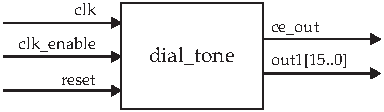
\includegraphics{../kapitel02/figures/dial_tone_fpga.pdf}
%	\caption{Structure of the generated \texttt{dial\_tone} module}
%	\label{fig:dial_tone_fpga}
%\end{figure}
%
%
%\begin{lstlisting}[language=Verilog,columns=flexible,caption= Extraction of the generated Verilog code,label=hdl_01]
%module dial_tone(...)
%
%always @(address_cnt_1)
%  ...
%  begin
%    case(address_cnt_1)
%      7'b0000000 : Sine_Wave1_out1 = 16'b0000000000000000;
%      7'b0000001 : Sine_Wave1_out1 = 16'b0000100000001001;
%      ...
%    endcase
%  end  
%  assign Add_add_cast = Sine_Wave_out1;
%  assign Add_add_cast_1 = Sine_Wave1_out1;
%  assign Add_add_temp = Add_add_cast + Add_add_cast_1;
%  assign Out1 = Add_add_temp[15:0];
%  
%endmodule  // dial_tone
%\end{lstlisting}
%
%Listing \ref{hdl_01} shows an extraction of the generated Verilog code for the dial tone example. The sine waves are generated by a lookup table and the output is assigned to the highest 16 bit of the sum of the sine waves. Figure \ref{fig:dial_tone_fpga} shows the structure of the generated Verilog module.
%
%\section{Overhead of Code Generation}
%\label{sec:overhead}
%
%The efficiency of generated code is still highly controversial in the development of radio systems. While some are complaining about the fact that the code is too slow baseband signal processing, others argue that there is no overhead. In this section, the processing time of the generated code was measured on different processing units under varying conditions like compilers or data types. It is furthermore compared with an unoptimized hand written code and an assembly-based optimized code. Parts of these measurements were also published in \cite{perf_overhead}.
%
%
%\subsection{Code Generation for GPPs}
%
%The benchmarks for generated C/C++ code were executed on an Intel Core 2 Duo CPU (P8400) with a clock frequency of \SI{2.28}{GHz}. The processor is working with a Windows 7 operating system and three compilers:
%\begin{itemize}
%	\item In the following the C/C++ compiler, which is integrated in Visual Studio 2005, is named \emph{VS}. The comparison with newer versions of the Visual Studio Express Edition showed no differences in speed. Therefore only this version is listed in the results.
%	\item The Local C Compiler in the following denoted as \emph{LCC} is a small open source C compiler, where in the benchmarks, version 2.4.1 is used.   
%	\item Intel Parallel Studio XE2011 integrates a C/C++ compiler in the development environment, which is especially suited for Intel architectures. The compiler is subsequently denoted as \emph{IPS}.
%\end{itemize}
%
%The C/C++ code was generated with Real Time Workshop version 7.6. For better readability and comparison with different processors, the benchmarks show, beside the time consumption of the evaluated code, also the number of cycles. These are calculated by the processing time multiplied with the processor frequency. Therefore, it is just a time scaling.
%
%Figure \ref{fig:empty_loop_gpp} shows the overhead that the generated code consumes after every \ac{ISR} due to scheduling, logging and status updates. This is the time the code remains in the gray boxes in figure \ref{fig:sample_frame}. It can be seen that the choice of the compiler dramatically influences the differences in processing times. The \ac{IPS} consumes less than a third of the time than the \ac{LCC}. The figure indicates also the influence of the frame size on the generated overhead. While the processing time of the non-functional code in figure \ref{fig:empty_loop_gpp} remains constant, the processing time for code inside the \texttt{model\_output} function increases with the frame size and leads to a better throughput in total.
%
%\begin{figure}[htbp]
%	\centering
%		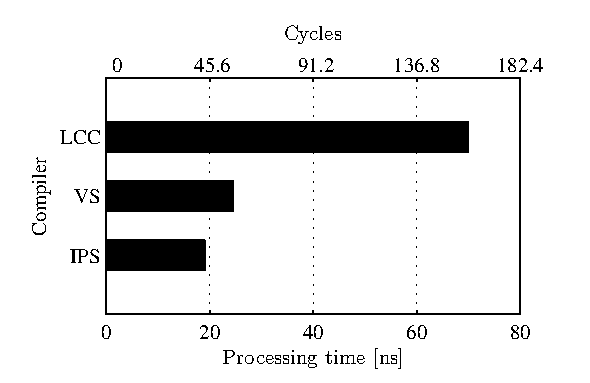
\includegraphics{../kapitel02/figures/empty_loop_gpp.pdf}
%	\caption{Processing times of the generated non-functional code, which was compiled with various compilers}
%	\label{fig:empty_loop_gpp}
%\end{figure}
%
%One of the essential signal processing functions in SDRs are \ac{FIR} filters\index{FIR filter}. Figure \ref{fig:fir_gpp} shows the benchmark of an \ac{FIR} filter compiled with the aforementioned compilers. To present values independent of the number of taps and frame size, the results are normalized to one input sample and one tap, leading in the best case to only one \ac{MAc} operation. Additionally to the named compilers, the data type (real or complex) and the code (hand written or generated) are compared. The results for the compilers from figure \ref{fig:empty_loop_gpp} are also valid for this benchmark. The \ac{VS} and \ac{IPS} produce the fastest code. The generated code consumes always less time than the hand written code. Note that the hand written code is not optimized in any sense except in the implementation of a circular buffer. The source code of the unoptimized hand written FIR filter can be found in appendix \ref{sec:app_FIR}. The fastest code is the generated code for an \ac{FIR} filter with real data and compiled with the \ac{IPS}. Only three cycles are consumed on the GPP per real tap and real sample. The processing time for a complex operation takes about ten cycles, which is also a good result, taking into account that the complex \ac{MAc} operation needs four real multiplications and two additions.
%
%\begin{figure}[htbp]
%	\centering
%		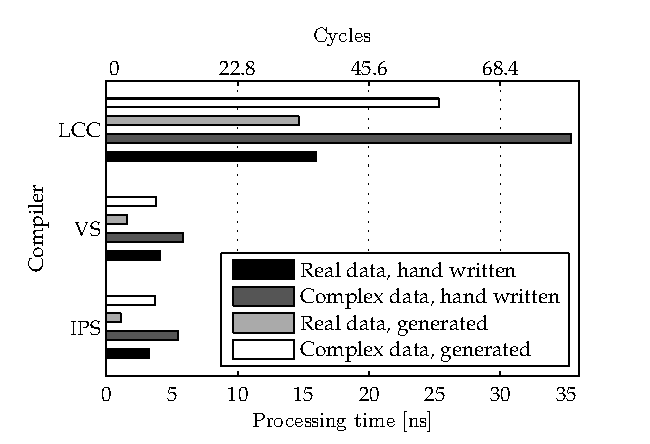
\includegraphics{../kapitel02/figures/fir_gpp.pdf}
%	\caption{Benchmark of an FIR filter on a GPP}
%	\label{fig:fir_gpp}
%\end{figure}
%
%Another important algorithm used in a waveform implementation is the \ac{FFT}\index{FFT}. Figure \ref{fig:fft_gpp} compares the processing times of an \ac{FFT} for \emph{generated code}, \emph{unoptimized hand written code} and an \emph{optimized code}. This optimized code comes from FFTW, which is a C subroutine library for calculating discrete Fourier Transforms. It is supported by an open software platform and is in performance comparable to machine-specific, vendor-optimized codes. The good performance is achieved by querying the parameters through the operating system and tuning the architecture automatically for the fastest results \cite{fftw_paper}. The unoptimized code is the straight implementation of the Cooley-Tukey algorithm, which can be found in appendix \ref{sec:app_03}.
%
%\begin{figure}[htbp]
%	\centering
%		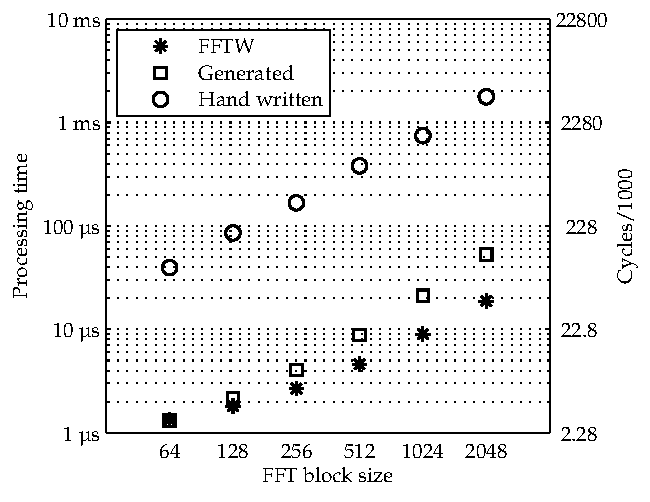
\includegraphics{../kapitel02/figures/fft_gpp.pdf}
%	\caption{Benchmark of the FFT on a GPP}
%	\label{fig:fft_gpp}
%\end{figure}
%
%For better comparability the compiler times are not included in the above results. The differences in the times for the compilers are in accordance to the previous results, which are shown in figure \ref{fig:empty_loop_gpp}. The input data are complex floating point vectors with a length according to a power of two. The hand written code is about thirty times slower than the generated and optimized code. They are varying over the FFT block size according to the benchmarks of the FFTW in \cite{fftw_bench}. There, it is shown, that the FFTW implementation achieves the best speed results with FFT sizes between 512 and 2048. The speed of the generated code does not fully reach the optimized FFTW implementation.
%
%
%
%\subsection{Code Generation for DSPs}
%
%The benchmarks for generated C code were measured with a C64x+ core on Texas Instrument's DM6446 system on chip, which is described in more details in section \ref{sec:SFF}. The processing times and cycles are in accordance with the GPP measurements when taking the scaling factor of the DSP's clock frequency of \SI{594}{MHz} into account. The C code is compiled with \ac{CCS} from the \ac{DSP} vendor \ac{TI}. Figure \ref{fig:empty_loop_dsp} shows an overhead of \SI{3.8}{\micro s} of the generated non-functional code. Referring to the number of cycles, this is about fifty times more than the non-functional code for the GPP. This is mainly caused by the underlying fixed point processor that has to deal with floating point code.
%
%\begin{figure}[htbp]
%	\centering
%		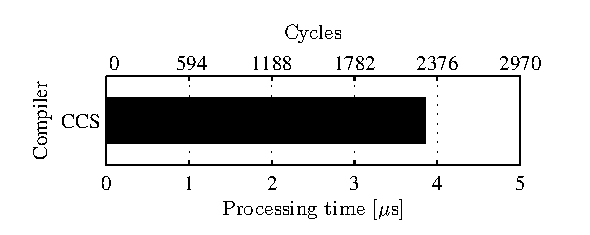
\includegraphics{../kapitel02/figures/empty_loop_dsp.pdf}
%	\caption{Overhead of the non-functional code on a DSP}
%	\label{fig:empty_loop_dsp}
%\end{figure}
%
%The performance loss of floating point code on a fixed point processor can also be seen in the benchmark of an \ac{FIR} filter\index{FIR filter} represented in figure \ref{fig:fir_dsp}. While the difference between floating point and fixed point arithmetic with hand written code makes a factor of ten, the generated fixed point code is about hundred times faster than the generated code dealing with floating point data types. The optimized code with a special library for digital signal processing comes from \ac{TI} and is only available in fixed point arithmetic. The generated fixed point code needs twice the time, which is not a bad result compared with the hand written, non-optimized code.
%
%\begin{figure}[htbp]
%	\centering
%		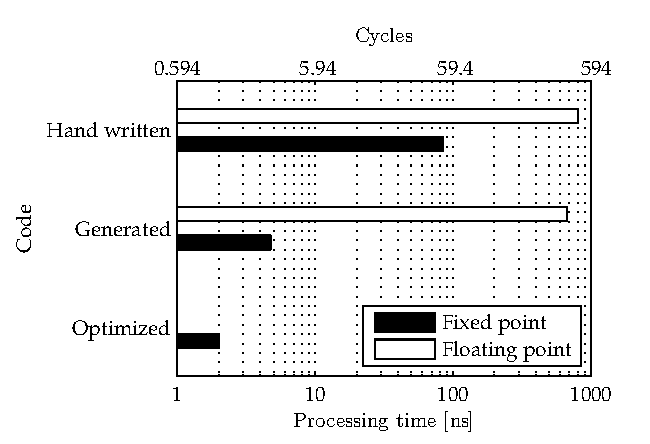
\includegraphics{../kapitel02/figures/fir_dsp.pdf}
%	\caption{Benchmark of an FIR filter on a DSP}
%	\label{fig:fir_dsp}
%\end{figure}
%
%Figure \ref{fig:fft_dsp} compares the results for the \ac{FFT}\index{FFT} for \emph{hand written code}, \emph{generated code} and the \emph{assembler optimized code} from TI's signal processing library. It has to be noted that the hand written code uses floating point arithmetic in contrast to the other code. This leads to the poor results, which are in processing time several decades slower than the optimized codes. The speed up for the optimized code is about four times higher than the generated C code.
%
%\begin{figure}[htbp]
%	\centering
%		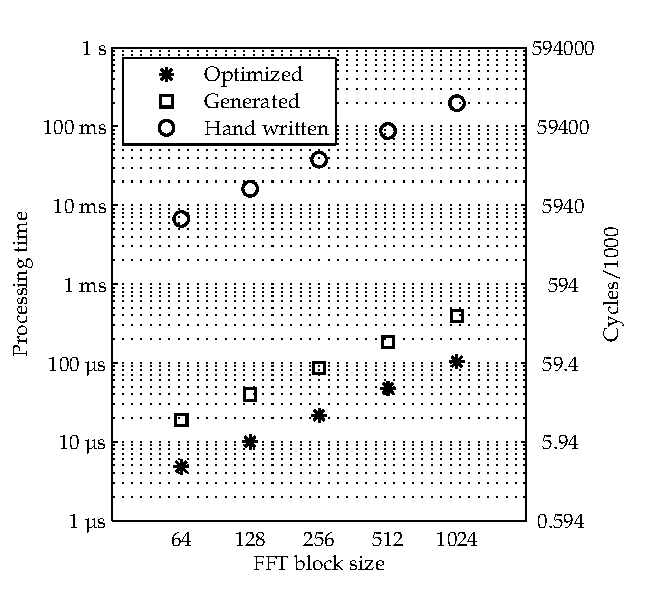
\includegraphics{../kapitel02/figures/fft_dsp.pdf}
%	\caption{Benchmark of the FFT on a DSP}
%	\label{fig:fft_dsp}
%\end{figure}
%
%
%\subsection{Code Generation for FPGAs}
%
%In contrast to the generated codes for \acp{DSP} and \acp{GPP}, the generated \ac{HDL} code creates no overhead for the system. The main task of the \ac{FPGA} on a \ac{SDR} is the adaptation of the DSP sample rate to the higher data rate of the \ac{DAC} and vice versa. Therefore, decimation and interpolation filters have to be realized. Figure \ref{fig:cic_fpga} shows the resource usage of interpolation filters with a \ac{CIC}\index{CIC filter} structure. The filters were implemented on a Virtex 4 FPGA from Xilinx with \acs{VHDL} \cite{virtex4} and on a Cylone FPGA from Altera with Verilog \cite{cyclone2}.
%
%\begin{figure}[htb]
%	\centering
%		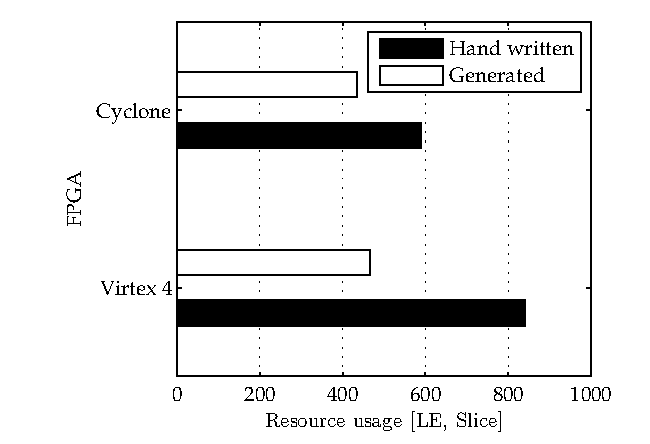
\includegraphics{../kapitel02/figures/cic_fpga.pdf}
%	\caption{Benchmark of a CIC decimation filter on different FPGAs}
%	\label{fig:cic_fpga}
%\end{figure}
%
%The interpolation factor was 128 and the bit lengths for input and output were 16. The bit length inside the filter increased to 44 due to bit pruning. The filter was implemented with four cascaded stages. Due to the different hardware architectures, the resource usage between both FPGAs can not be compared. The FPGAs from the company Altera are based on \ac{LE}\index{Logic Element}, which mainly consists of one programmable register, one carry chain and one \ac{LUT} with four inputs. This is different from the Xilinx approach. The smallest logic block is named ``slice''\index{Slice}, comprising two \acp{LUT} with four inputs, one carry chain and two programmable registers. Therefore, the resource usage of the filter was measured in \acp{LE} for the Cyclone and in slices for the Virtex FPGA. The generated code is smaller in the sense of space than the hand written code but the difference is not as dominating as in the previous sections.
%
%
%Beside \ac{CIC} filters, also \ac{FIR}\index{FIR filter} filters, used for decimation in time, are benchmarked. Figure \ref{fig:fir2_fpga} shows the difference between an optimized halfband decimation filter in comparison to the generated polyphase decimation filter. The filter length was 31 but due to the coefficient properties, only eight multiplications were needed. The other coefficients were zero. Furthermore, due to the symmetry of the filter some coefficients were equal. The generated filter did not recognize this symmetry and hence the possibilities to use this for optimization.
%
%\begin{figure}[htbp]
%	\centering
%		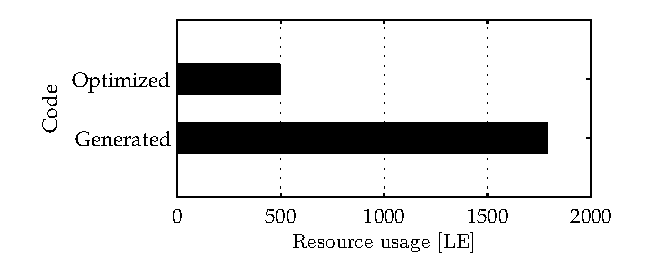
\includegraphics{../kapitel02/figures/fir2_fpga.pdf}
%	\caption{Comparison of the resource usage for a 31-tap halfband filter}
%	\label{fig:fir2_fpga}
%\end{figure}
%
%To get an overview how the number of taps correlate with the resource usage in generated code, Figure \ref{fig:fir_fpga} shows the used \acp{LE} of a decimate by two filter. The bit length of input and output signal as well as the filter coefficients was 16 bit, the bit length of the accumulator was 32 bit. The results of figure \ref{fig:fir_fpga} were measured on a Cyclone FPGA without hardware multipliers.
%
%\begin{figure}[htbp]
%	\centering
%		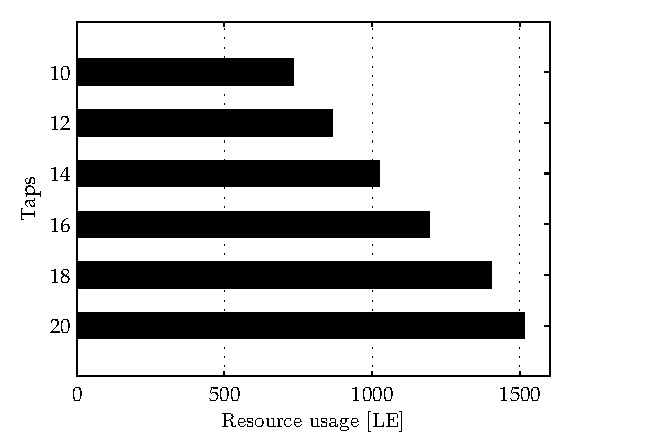
\includegraphics{../kapitel02/figures/fir_fpga.pdf}
%	\caption{Comparison of the resource usage of an FIR decimation filter with various tap lengths}
%	\label{fig:fir_fpga}
%\end{figure}
%
